\section{Covariance matrix spectrum}
The covariance matrix is defined as 
\[
M_{\alpha,\beta}=\frac{1}{N}\sum_iS_i^{(\alpha)}S_i^{(\beta)}-
\frac{1}{N}\sum_iS_i^{(\alpha)}\frac{1}{N}\sum_jS_j^{(\beta)}
\]
where $\alpha$, $\beta$ are replicas of the same disorder configuration, 
but from different Markov chains.

One can then examine the spectrum use Singular Value Decomposition, since
the covariance is always a positive definite matrix. 
We then calculate the average of the singular values over different disorder 
configurations. 

\begin{figure}[ht]
  \centering
  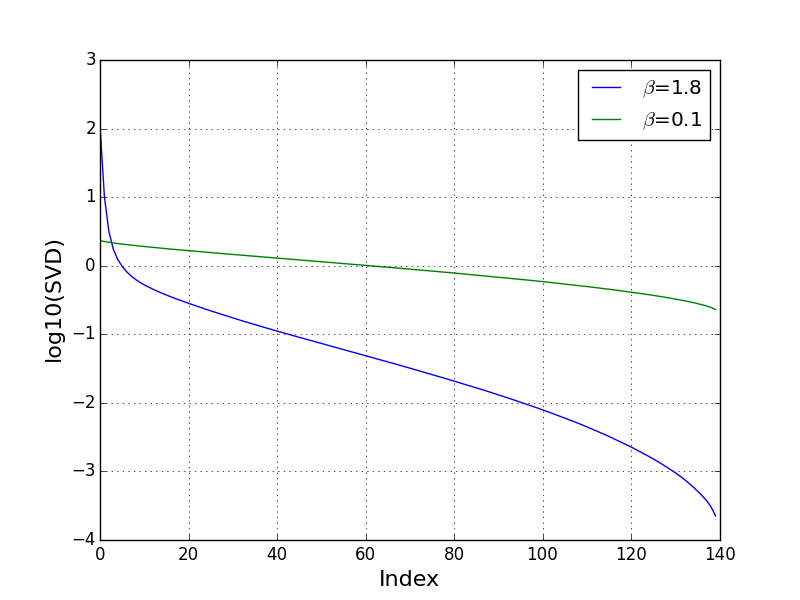
\includegraphics[width=0.6\textwidth]{img/matrix/svd_data.png}
  \caption{Singular values of covariance matrix for 3D EA model, h=0, L=8, 
averaged over 1000 disorder realizations. 
Each matrix is formed from 140 samples of the same disorder realizations.}
  \label{fig:exp}
\end{figure}

FIG. \ref{fig:exp} shows the singular value calculated with this method, using
the data we gathered on Shelob.

\section{Different phases/scenarios}
Here we discuss a few possible scenarios of this model.

\begin{enumerate}
\item{High temperature or paramagnetic phase}

The diagonal elements in the covariance matrix would be 
\[M_{\alpha,\alpha}=1-(\frac{1}{N}\sum_is_i^{(\alpha)})^2 \sim 1-O(N^{-1})\]
the off diagonal elements would be 
\[M_{\alpha,\beta\neq\alpha}=\frac{1}{N}\sum_iS_i^{(\alpha)}S_i^{(\beta)}-
\frac{1}{N}\sum_iS_i^{(\alpha)}\frac{1}{N}\sum_jS_j^{(\beta)}
\sim O(N^{-1/2})
\]

In general the matrix is not singular, and the distribution should look like the
$\beta=0.1$ line in FIG \ref{fig:exp}.


\item{Ferromagnetic phase}

In the ferromagnetic limit, the system has two symmetric degenerate states.
All the replicas should then fall into one of these states.
The vacuum cancels the contribution from the overlap, and therefore
all elements in the matrix would be close to zero.


\item{Droplet picture}

There is only a pair of degenerate ground states in the Droplet picture. 

In this case, the matrix would be composed with only $+1$ and $-1$, since 
the vacuum term is zero on average.
 
The matrix is singular and has only 1 finite singular value.

\begin{figure}[ht]
  \centering
  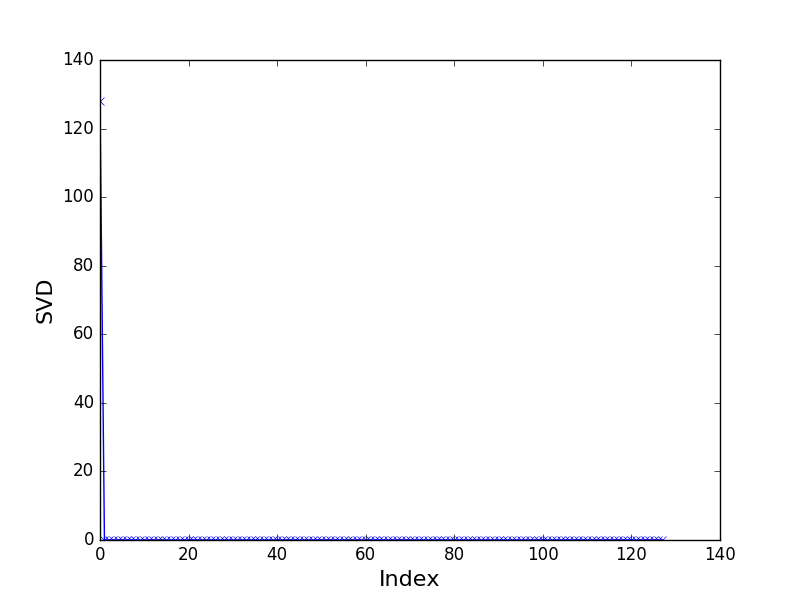
\includegraphics[width=0.6\textwidth]{img/matrix/eigDropletTheo.png}
  \caption{Theoretical distribution for the eigenvalues of the Droplet model,
N=128.}
  \label{fig:dropTheo}
\end{figure}





\item{Replica Symmetry Breaking (RSB) picture}

In RSB, there is a tree-like hierarchy in the structure of phase space.
We can assume the overlap also follows a tree structure. 

\begin{figure}[ht]
  \centering
  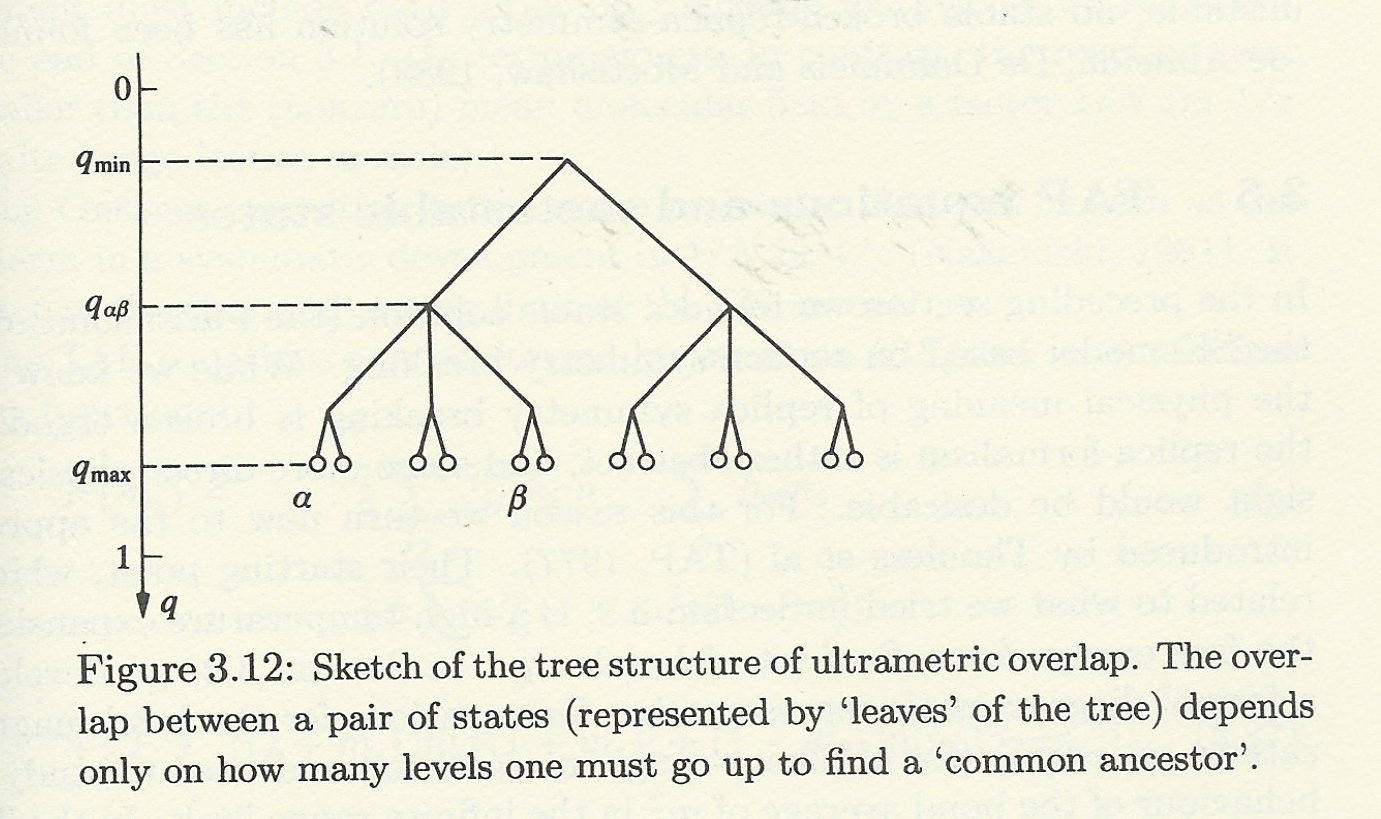
\includegraphics[width=0.8\textwidth]{img/matrix/tree.png}
  \caption{Illustration of the tree structure. From Fischer \& Hertz, Spin Glasses, page 93}
  \label{fig:tree}
\end{figure}


For simplicity, we used a binary tree to represent the structure of states. 
In equilibrium, all replicas should fall onto one of the leaves of the binary tree. 

The depth of the tree determines the degree of degeneracy of ground state. 
A larger depth is favorable since RSB predicts an infinite number of 
degenerate ground states in the thermal dynamic limit. We used 32,
 which corresponds to $2^{32}$ ground states.


The distribution of $q$ levels shows the similarity of ground states.
We start with a power-law distribution. 

We can then use this tree structure to investigate the behavior of covariance matrix
in the RSB picture.

To mimic the simulation, we generate multiple sets of samples. Each set contains
140 samples. Each sample is a ground state, i.e, a random leaf of the binary tree. 
We can then find the overlap between each pair of samples 
from their position on the tree, form the covariance
matrix and calculate the singular values. 
We average over 2000 sets of samples.

\begin{figure}[ht]
  \centering
  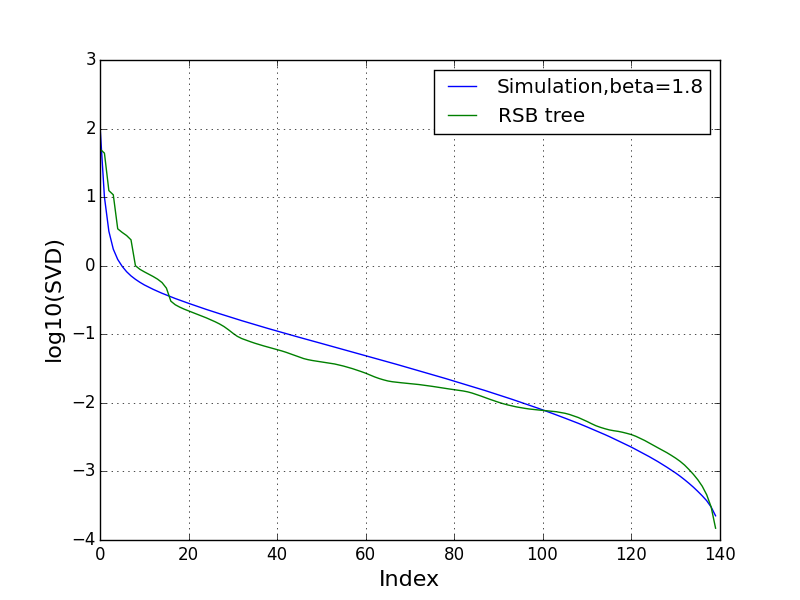
\includegraphics[width=0.6\textwidth]{img/matrix/svd_compare_rsb.png}
  \caption{Comparison between the simulation data and the RSB tree test. For the RSB tree,
we used a tree depth of 32, $q_{max}=1.0$, $q_{min}=0.2$, power-law distributed $q$ levels.}
  \label{fig:compare}
\end{figure}


We see some interesting similarities in the distribution between the
singular values we generated using this method, and the singular values we 
calculated from real simulation data.

\end{enumerate}

\section{Distribution of $\lambda$}

To understand the spectrum better, we look at some of the distribution of 
a few eigenvalues. Here $\lambda_i$ stands for the $i$th largest eigenvalue.
 
\begin{figure}[ht]
\centering
  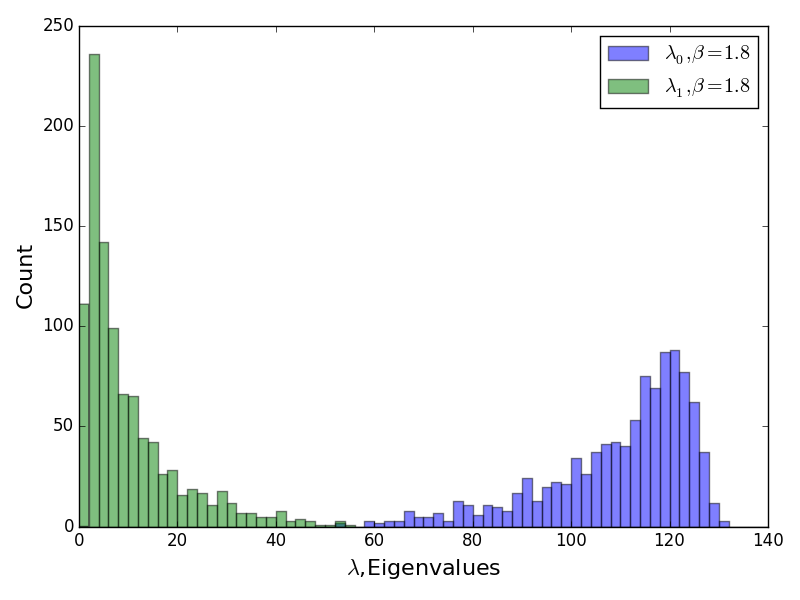
\includegraphics[width=0.7\textwidth]{img/matrix/eigHist1.png} 
\caption{Histogram of the largest two eigenvalues, $\beta=1.8$. The distribution 
is not symmetrical and non-Gaussian.}
\label{fig:hist1}
\end{figure}

\begin{figure}[ht]
\centering
  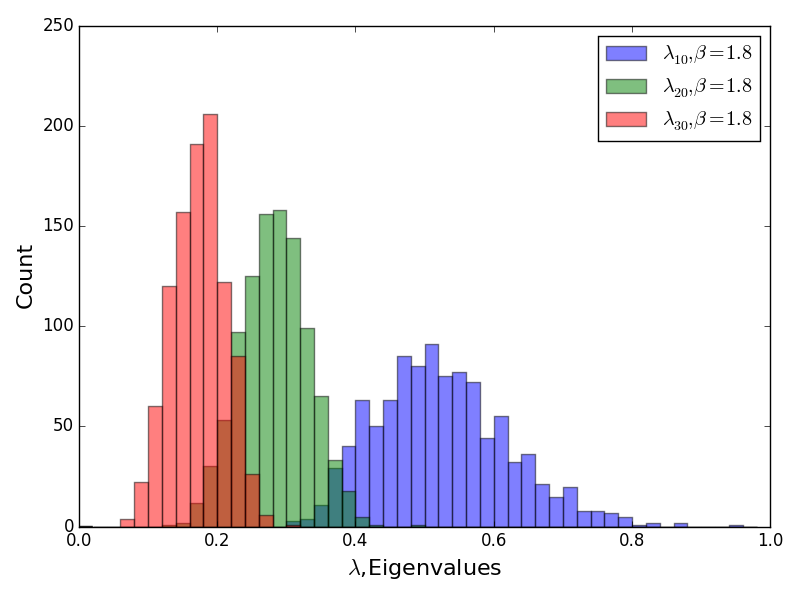
\includegraphics[width=0.7\textwidth]{img/matrix/eigHist2.png} 
\caption{Histogram of the three eigenvalues, $\lambda_{10}$,$\lambda_{20}$, 
$\lambda_{30}$, $\beta=1.8$.}
\label{fig:hist2}
\end{figure}

\begin{figure}[ht]
\centering
  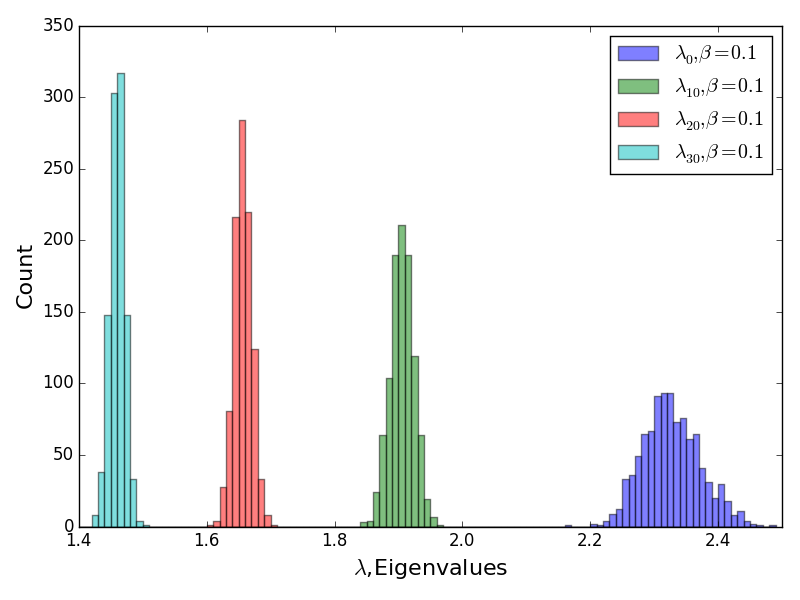
\includegraphics[width=0.7\textwidth]{img/matrix/eigHist3.png} 
\caption{Histogram of the eigenvalues, $\lambda_0$,$\lambda_{10}$,$\lambda_{20}$, $\lambda_{30}$, $\beta=0.1$.}
\label{fig:hist3}
\end{figure}

From the distribution, we see that the distribution of first few largest 
eigenvalues at $\beta=1.8$ (FIG.\ref{fig:hist1}) is not Gaussian. 
All the other data are almost normally distributed (FIG.\ref{fig:hist2},\ref{fig:hist3}).

Take $\lambda_1$, $\beta=1.8$ for example. It seems that for a portion of realizations,
$\lambda_1$ is much larger than the smaller eigenvalues, i.e. there are more 
than one large eigenvalues.
For other
realizations $\lambda_1$ is on the same order and has similar distribution with 
the smaller eigenvalues, i.e. there is only one large eigenvalue. 


The disorder realizations can be very different from each other. 
Previously for the droplet model,
we only looked at one disorder configuration, and this may not be enough. 
We need to do more realizations and examine the distribution/average to see
if all the realizations have only 1 large eigenvalue. 

The largest eigenvalue of the covariance matrix is the variance in the 
direction that the data varies the most. The second largest eigenvalue is the 
the greatest variance among the directions that are orthogonal 
to the first eigenvector, and so on. So if there is only one large eigenvalue,
this means there is only one pair of states that are dominant, since the system
only varies in that one direction. In any other direction, the energy penalty 
to make a move is much higher and thus the variance is much smaller, hence 
a smaller eigenvalue.

Counting degenerating ground states is possible for some toy systems. 
For example, for a system of three spins in a triangle that have nearest 
neighbor interaction. If all interaction are ferromagnetic, then the system is
ferromagnetic, and has only two degenerate states. This corresponds to the 
case with only one dominant eigenvalue.


Consider the same system with all anti-ferromagnetic bonds. Then the system has
six degenerate ground states, with a set of four possible values of 
overlap between each other. The corresponding covariance matrix has two finite 
eigenvalues. 

Another example is a system of four spins in a square, with three 
anti-ferromagnetic bond and one ferromagnetic bond.
Then the system has eight degenerate ground states, with a set of nine possible 
values of overlap between each other. The corresponding covariance matrix has 
three finite eigenvalues. 


%I think the number of degenerate ground states/possible values of overlap is
%related to the number of large eigenvalues. However, more investigation on the
%droplet model is necessary. I have received the code from Ka-Ming and I'll
%do more simulations on this. 

\section{Data from Droplet model}
We ran the model with a weakly correlated random disorder (van Hemmen model),
where
\[
J_{ij}=\eta_i\zeta_j+\zeta_i\eta_j
\]

The distribution of q is shown in Fig. \ref{fig:q_droplet}. 
\begin{figure}[ht]
  \centering
  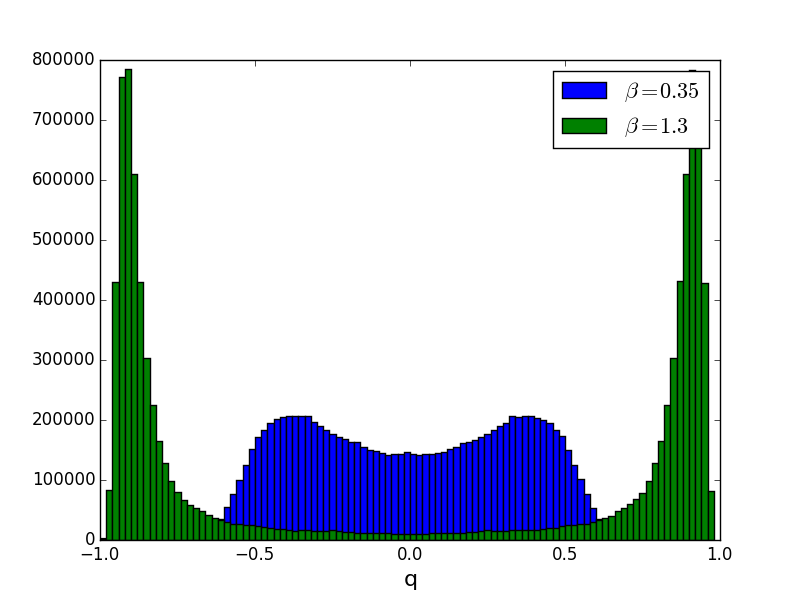
\includegraphics[width=0.8\textwidth]{img/matrix/q_dist_droplet.png}
  \caption{The distribution of q in the droplet model.}
  \label{fig:q_droplet}
\end{figure}


The distribution of eigenvalues is shown in Fig. \ref{fig:eigDroplet}.

\begin{figure}[ht]
  \centering
  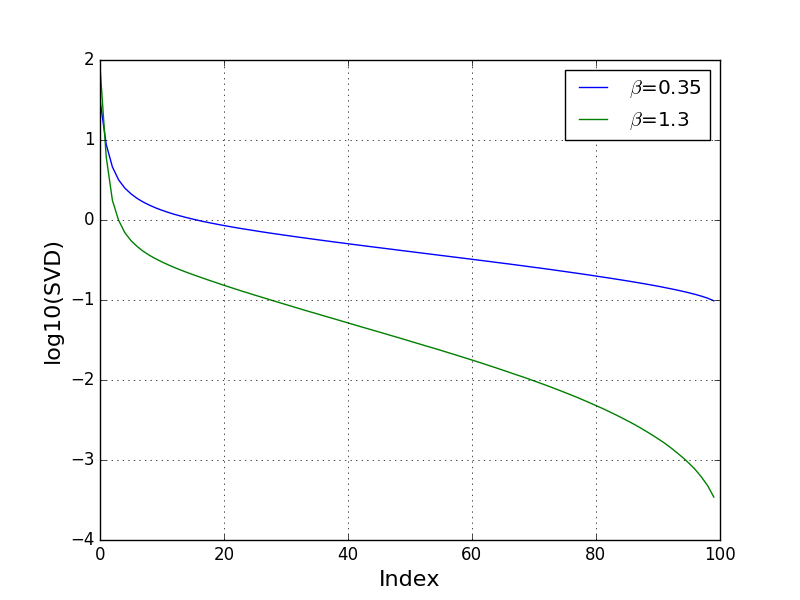
\includegraphics[width=0.6\textwidth]{img/matrix/eigDroplet.png}
  \caption{Singular values of covariance matrix for 3D droplet model, h=0, L=8, 
averaged over 1000 disorder realizations. 
Each matrix is formed from 100 samples of the same disorder realizations.}
  \label{fig:eigDroplet}
\end{figure}

The histogram of the largest few eigenvalues is shown in Fig. \ref{fig:eigDropletDist}.

\begin{figure}[ht]
  \centering
  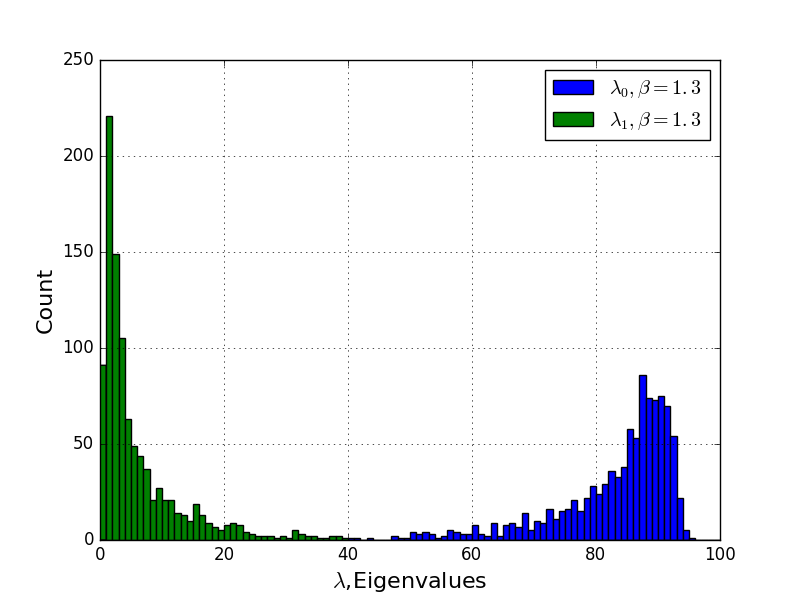
\includegraphics[width=0.6\textwidth]{img/matrix/eigDropletDist.png}
  \caption{Histogram of the two largest eigenvalues of covariance matrix for 3D droplet model, h=0, L=8, 
averaged over 1000 disorder realizations. 
Each matrix is formed from 100 samples of the same disorder realizations.}
  \label{fig:eigDropletDist}
\end{figure}

Comparing the result from Droplet model and EA model, we do not see much difference.

Even there is a difference between the Droplet model and EA model, it seems 
the system size we use is not large enough to show it.

\section{Data from RSB model }
We use the Sherrington-Kirkpatrick Model here:
\[
H=-\frac{1}{\sqrt{N}}\sum_{1\le i \le j \le N} J_{ij}\sigma_i\sigma_j
\]
This model has an equilibrium phase transition at $T_c=1$. 


The distribution of eigenvalues is shown in Fig. \ref{fig:eigRSB}.

\begin{figure}[ht]
  \centering
  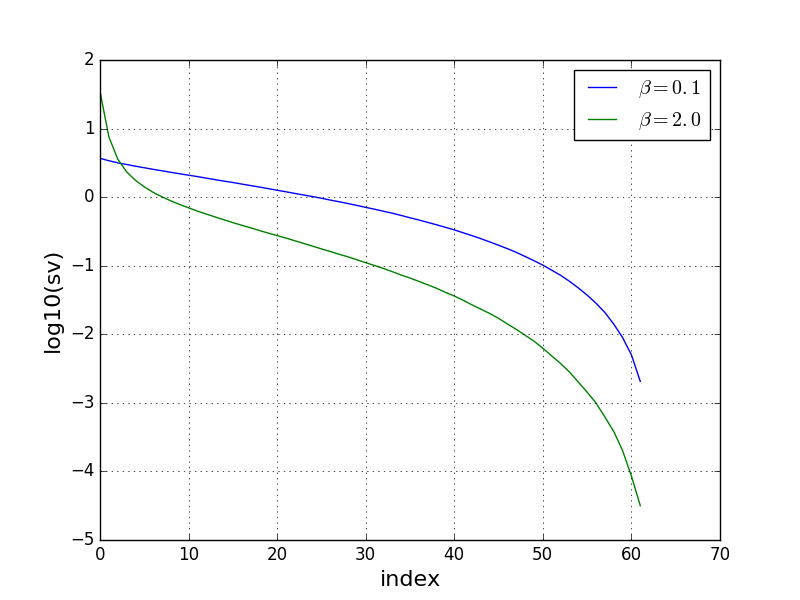
\includegraphics[width=0.6\textwidth]{img/matrix/svdDistRSB.png}
  \caption{Singular values of covariance matrix for SK model, h=0, N=64, 
averaged over 280 disorder realizations. 
Each matrix is formed from 64 samples of the same disorder realizations.}
  \label{fig:eigRSB}
\end{figure}

At low temperature, the data seems very similar to that of EA model and Droplet 
model.


\begin{figure}[ht]
  \centering
  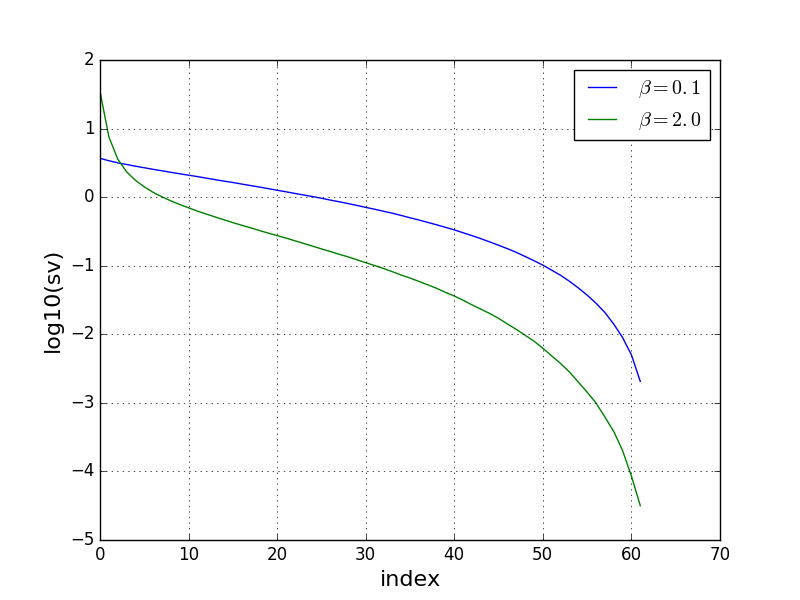
\includegraphics[width=0.6\textwidth]{img/matrix/svdDistRSB.png}
  \caption{Singular values of covariance matrix for SK model, h=0, N=64, 
averaged over 280 disorder realizations. 
Each matrix is formed from 64 samples of the same disorder realizations.}
  \label{fig:eigRSB}
\end{figure}

\section{Comparison among three models}
We further inspect the temperature dependency of the eigenvalues for different
models,by plotting the (second largest eigenvalue of the covariance matrix / linear size 
of the covariance matrix) vs ($\beta/\beta_c$) for three different models, where
$\beta_c$ is the critical beta for each model, as shown in Fig.\ref{fig:eig0} 
and Fig.\ref{fig:eig1}.

\begin{figure}[ht]
  \centering
  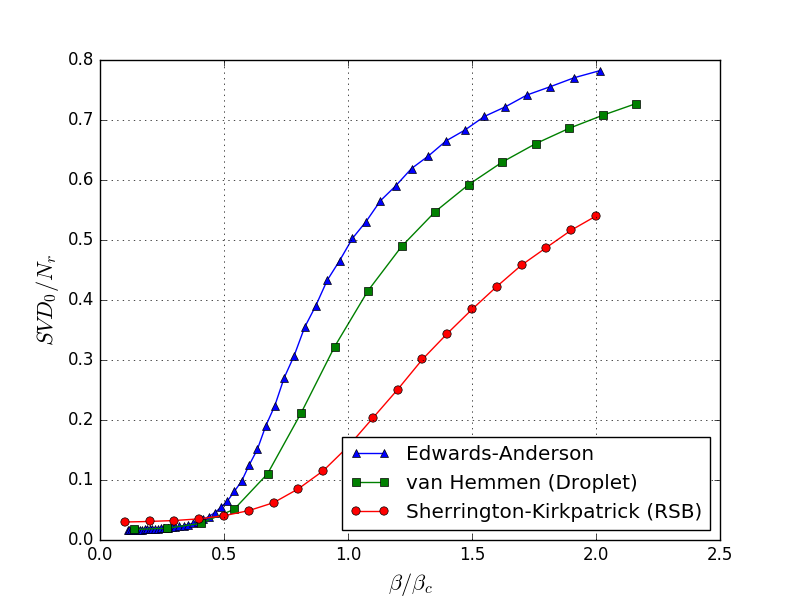
\includegraphics[width=0.6\textwidth]{img/matrix/svd0_vs_beta.png}
  \caption{Temperature dependency of the largest eigenvalue, for EA, droplet and RSB model.}
  \label{fig:eig0}
\end{figure}


\begin{figure}[ht]
  \centering
  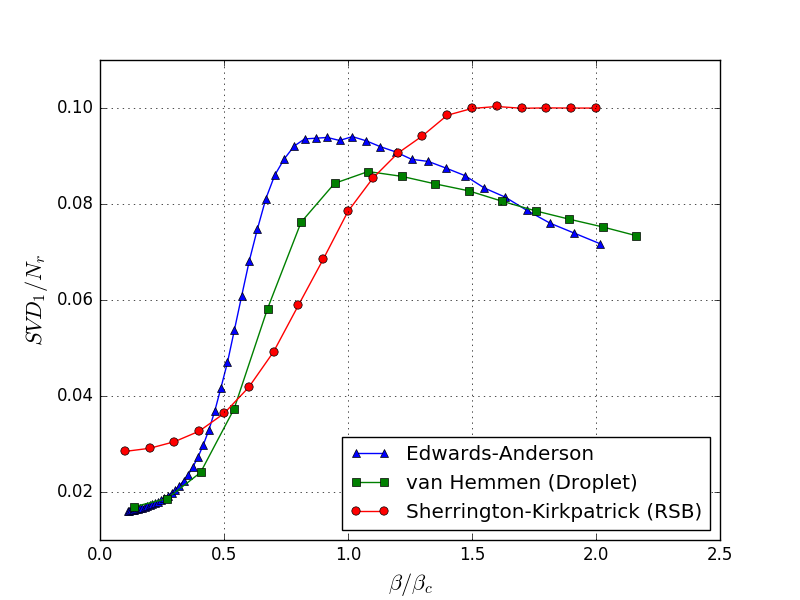
\includegraphics[width=0.6\textwidth]{img/matrix/svd1_vs_beta.png}
  \caption{Temperature dependency of the second largest eigenvalue, for EA, droplet and RSB model.}
  \label{fig:eig1}
\end{figure}

At first glance, the second largest eigenvalue reveals a big difference among 
the three models. The assumption is that the droplet picture has a simple 
structure in its phase space, thus, all eigenvalues except the largest will 
converge to zero at zero temperature, while the RSB picture has a rich structure 
in the phase space and the second largest eigenvalue will persist. 
From the figure, it may seem the data for EA model is more droplet-like. They both 
have a peak near the critical beta and goes down at the lower temperature.
However, when going into lower temperatures, we see that the second largest 
eigenvalue for SK model shows a similar trend, by decreasing at lower temperatures.

\begin{figure}[ht]
  \centering
  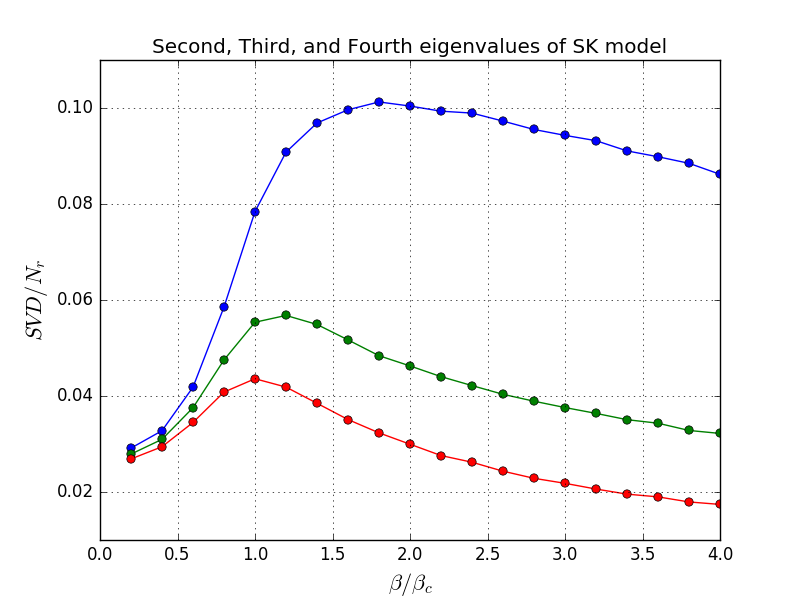
\includegraphics[width=0.6\textwidth]{img/matrix/eigenvalues_rsb.png}
  \caption{The second, third and fourth largest eigenvalues for RSB model vs
$\beta/\beta_c$.}
  \label{fig:eigRSB2}
\end{figure}


In conclusion, the data from the study on the covariance is not conclusive to 
discriminate the models and decide the nature of the spin glass phase.

%%% Local Variables:
%%% mode: latex
%%% TeX-master: t
%%% End:
